\section{Detección y corrección de errores y avisos}

\paragraph{}Importado el proyecto para el entorno de desarrollo \textbf{Eclipse} y tras pasarle el plugin \textbf{Metriculator}, vemos que cumple las condiciones para nuestra práctica al pasar tanto las métricas de Mccabe y LSLOC por lo que nos disponemos como siguiente paso a solventar los errores y warnings ofrecidos por su compilación.

\paragraph{}Tras una primera compilación del proyecto en Eclipse, se nos informa de que hay dos errores. A continuación, una captura de pantalla de la consola de Eclipse:

\begin{figure}[H]
	\centering
	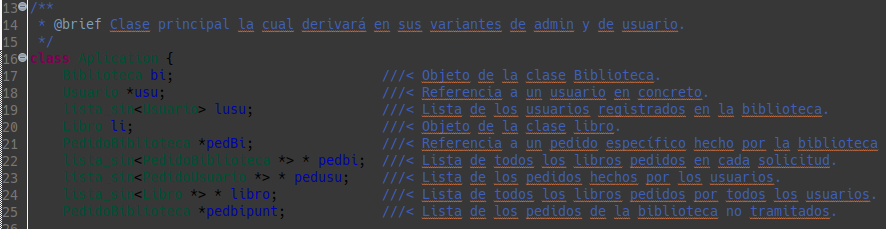
\includegraphics[scale=0.3]{img/captura2.png}
	\caption{Captura de pantalla de la consola de Eclipse}
	\label{captura1}
\end{figure}

\paragraph{}Además, dejamos también una captura de pantalla de la pestaña “Problems” de Eclipse:

\begin{figure}[H]
	\centering
	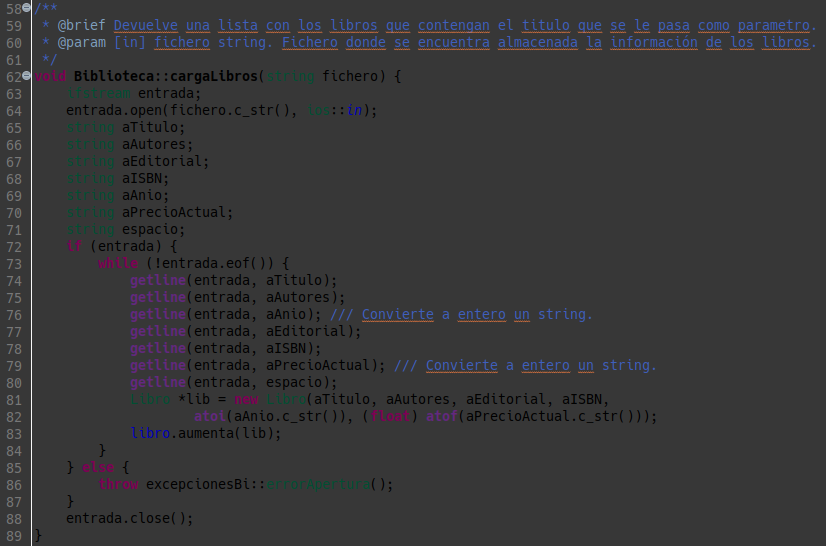
\includegraphics[scale=0.3]{img/captura1.png}
	\caption{Captura de pantalla de la pestaña "problems" de Eclipse}
	\label{captura2}
\end{figure}

\paragraph{}El primer error se sitúa en el archivo “PedidoBiblioteca.h”, en la línea 6. Este consiste en un error de escritura del nombre del archivo en el include; “fecha” debe de tener su primera letra en mayúscula para que sea reconocido. A continuación, dos capturas de pantalla: una con el error sin resolver y otra con el error resuelto.

\begin{figure}[H]
	\centering
	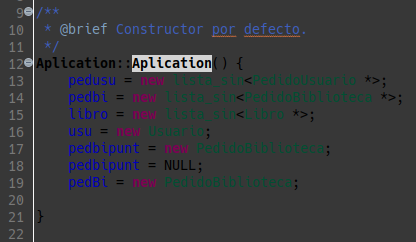
\includegraphics[scale=1]{img/captura3.png}
	\caption{Error sin resolver}
	\label{captura3}
\end{figure}

\begin{figure}[H]
	\centering
	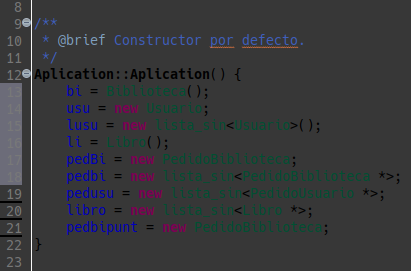
\includegraphics[scale=1]{img/captura4.png}
	\caption{Error resuelto}
	\label{captura4}
\end{figure}

\paragraph{}Tras corregir este error, volvemos a realizar una compilación del proyecto, y nos surgen los siguientes errores:

\begin{figure}[H]
	\centering
	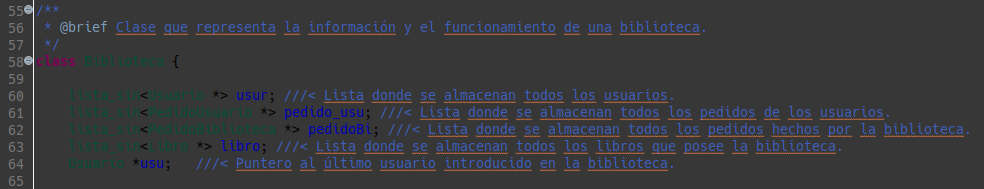
\includegraphics[scale=0.45]{img/captura5.png}
	\caption{Captura de pantalla de la consola de Eclipse}
	\label{captura5}
\end{figure}

\paragraph{}Volvemos a tener el mismo error, pero en el archivo “Fecha.cpp”, por lo que lo corregimos de la misma manera:

\begin{figure}[H]
	\centering
	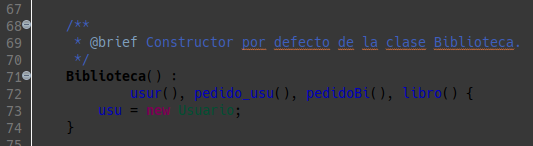
\includegraphics[scale=0.47]{img/captura6.png}
	\caption{Captura de pantalla de la pestaña "problems" de Eclipse}
	\label{captura6}
\end{figure}

\begin{figure}[H]
	\centering
	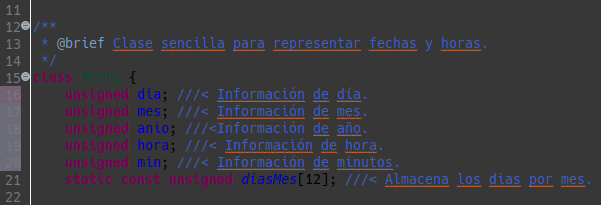
\includegraphics[scale=1]{img/captura7.png}
	\caption{Error sin resolver}
	\label{captura7}
\end{figure}

\begin{figure}[H]
	\centering
	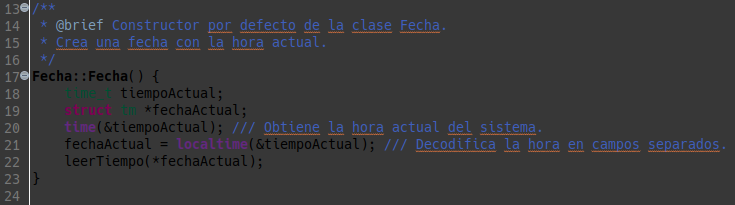
\includegraphics[scale=1]{img/captura8.png}
	\caption{Error resuelto}
	\label{captura8}
\end{figure}

\paragraph{}Una vez resuelto este error, volvemos a compilar el proyecto y ahora tan solo nos aparecen dos avisos, como se puede observar en la siguiente captura de pantalla:

\begin{figure}[H]
	\centering
	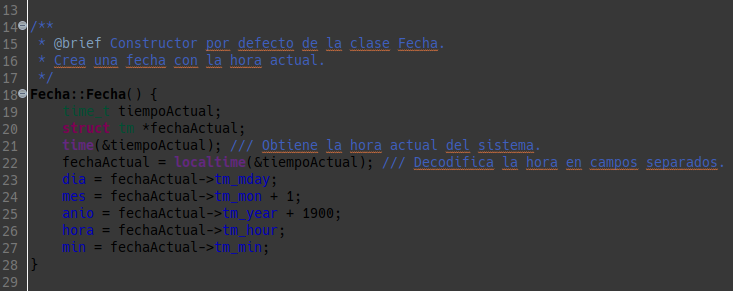
\includegraphics[scale=0.48]{img/captura9.png}
	\caption{Captura de pantalla de la pestaña "problems" de Eclipse}
	\label{captura9}
\end{figure}

\paragraph{}El primer aviso se encuentra en el archivo “PedidoBiblioteca.h”, en la línea 23, y nos dice que el atributo “num” no ha sido inicializado dentro del constructor por copia de “PedidoBiblioteca”. El aviso se resolvería asignándole el valor del atributo num del objeto pasado por referencia. A continuación, dos capturas de pantalla: en una se muestra el aviso sin resolver y en la otra el aviso resuelto.

\begin{figure}[H]
	\centering
	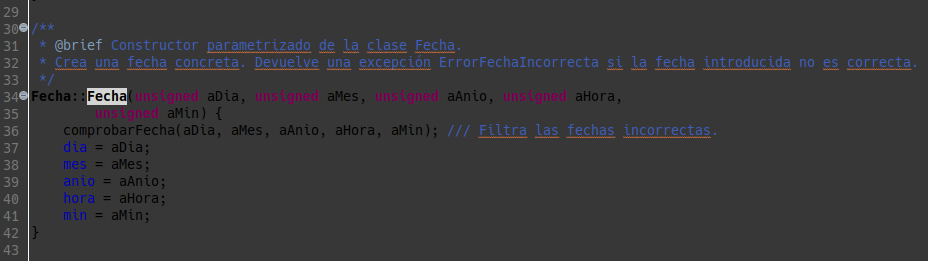
\includegraphics[scale=0.85]{img/captura10.png}
	\caption{Error sin resolver}
	\label{captura10}
\end{figure}

\begin{figure}[H]
	\centering
	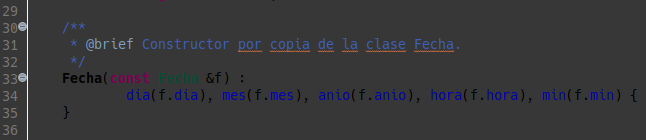
\includegraphics[scale=1]{img/captura11.png}
	\caption{Error resuelto}
	\label{captura11}
\end{figure}

\paragraph{}El segundo aviso nos dice que la autocomparación siempre se evalúa como falsa. Este aviso se encuentra en el archivo “PedidoUsuario.h”, en la línea 31. A continuación, una captura de pantalla para poder entender a qué se refiere:

\begin{figure}[H]
	\centering
	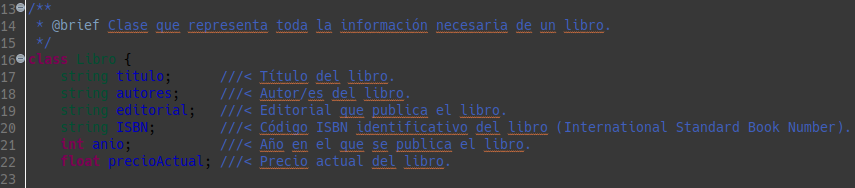
\includegraphics[scale=1]{img/captura12.png}
	\caption{Error sin resolver}
	\label{captura12}
\end{figure}

\paragraph{}Se puede observar que “this->prioridad” y “prioridad” hacen referencia al mismo atributo, por lo tanto, siempre se devolverá falso. Para corregir este aviso es necesario que se compare “this->prioridad” con el atributo prioridad del objeto que se pasa por referencia. A continuación, dejamos una captura de pantalla con el aviso solventado:

\begin{figure}[H]
	\centering
	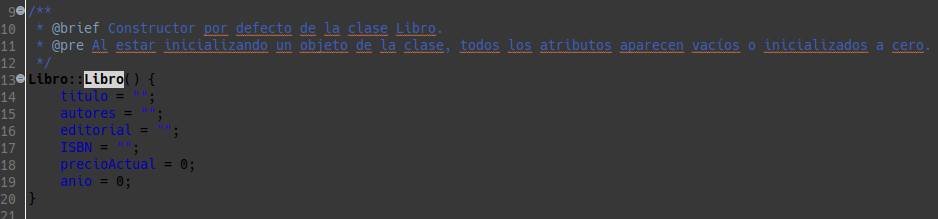
\includegraphics[scale=0.98]{img/captura13.png}
	\caption{Error resuelto}
	\label{captura13}
\end{figure}

\paragraph{}Una vez corregidos los dos avisos, volvemos a realizar una compilación del proyecto y esta vez no se detecta ningún error ni aviso, por lo que hemos finalizado.

\begin{figure}[H]
	\centering
	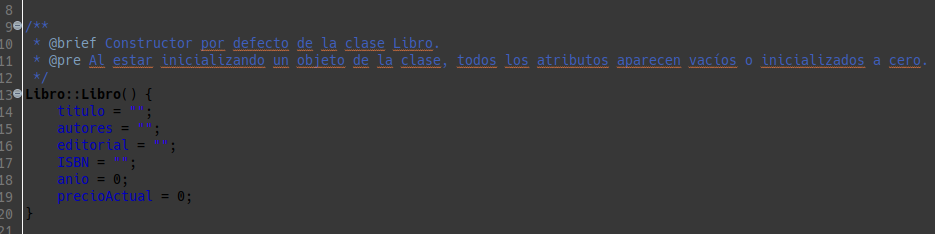
\includegraphics[scale=0.39]{img/captura14.png}
	\caption{Captura de pantalla de la consola de Eclipse}
	\label{captura14}
\end{figure}



\newpage